\chapter{RD53A}

Il progetto di RD53A è stato approvato nell'autunno del 2015, dopo la revisione da parte delle collaborazioni ATLAS, CMS e RD53A. Nel 2016 è iniziata la progettazione del chip, con RD53A si vuole dimostrare la possibilità di utilizzare tecnologia CMOS  in 65 nm per l'aggiornamento in vista della fase ad alta luminosità di ATLAS e CMS, e quindi la tolleranza al danneggiamneto da radiazioni, soglie di lavoro basse e stabili nel tempo, capacità di gestire un alto flusso di particelle incidenti e l'utilizzo di trigger veloci. 
RD53A non deve essere inteso come il prodotto finale, infatti possiede molte modifiche di desing utili solo in una prima fase di test, ad esempio al suo interno sono presenti tre diversi front-end (FE), già questo causa una non uniformità del chip. 
Questo chip è la base di partenza per arrivare al progetto finale, in cui sarà scelto uno dei front end e sarà utilizzato uniformemente su tutta la matrice di pixel. In RD53a la matrice di pixel ha 400 colonne e 192 righe, nel progetto finale si avrà un aumento del numero di pixel, infatti il sistema di alimentazione e di contropolarizzazione dei pixel è progettato per un numero di righe massimo pari a 384, figura \ref{RD53ALayout}.
\begin{figure}
\centering
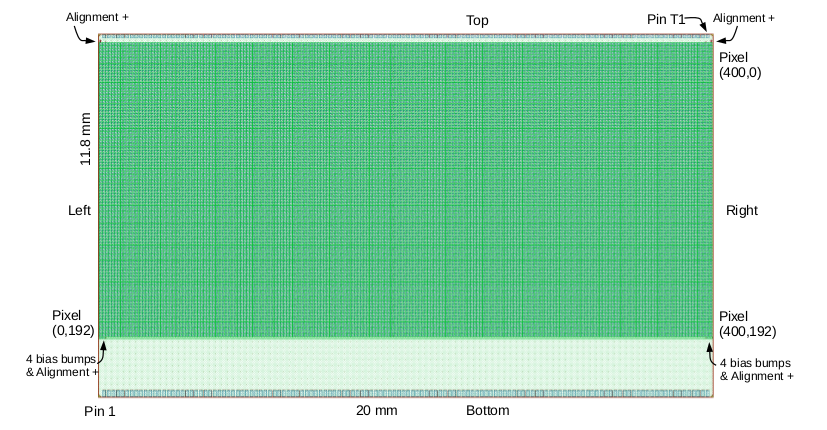
\includegraphics[scale=.4]{Immagini/RD53ALayout}
\caption{RD53A layout. Il chip è largo 20mm per 400 pixel e l'altezza è 11.8 mmm per 192 pixel.}
\label{RD53ALayout}
\end{figure}

%Floorplan
%RD53A uses a 9 metal layer stack, consisting of 7 thin, 1 thick and 1 ultra-thick metal layers.
%In addition, the 28K AP layer is also used for power lines distribution. In Fig. 2 and Fig. 3 the
%layout and functional view of RD53A floorplan are shown. The sensitive area of the chip is placed
%at the top of the chip and is arranged as a matrix of 192 x 400 pixels of 50 μm × 50 μm. At
%the top is a row of test pads for debugging purposes, which should be removed in a production
%chip. The peripheral circuitry is placed at the bottom of the chip and contains all global analog and
%digital circuitry needed to bias, configure, monitor and readout the chip. The wire bonding pads are
%organized as a single row at the bottom chip edge and are separated from the first row of bumps by
%1.7 mm in order to allow for wire bonding after sensor flip-chip (Sec. 4). However, the wire bond
%pads are also designed compatible with Thru-Silicon Via post processing.
%The pixel matrix is built up of 8 by 8 pixel cores. The 64 front ends within a core are placed as
%16 so-called analog islands with 4 fronts ends each, which are embedded in a flat digital synthesized
%“sea” as shown in Fig. 4. The circuitry around each island is not identical but depends on the
%placement of gates by the synthesis tool. Prototype tests have shown that, within the digital/analog
%isolation scheme used, this approach does not introduce any visible systematic differences between
%islands. Furthermore, a core is small enough that it can be checked with a transistor level analog
%simulation. In the chip periphery, all the analog building blocks are grouped in a macroblock called
%Analog Chip Bottom (ACB), which is fully assembled and characterized in an analog environment
%(Sec. 8). All the building blocks have been previously prototyped, tested and characterized in
%radiation environment at least up to 500 Mrad TID. The ACB block is surrounded by a synthesized
%block, called Digital Chip Bottom (DCB), which implements the Input, Output and Configuration
%digital logic, as described in (Sec. 7) and (Sec. 9).
\section{Single Chip Card}

\section{Misure con chip}
\begin{figure}
\centering
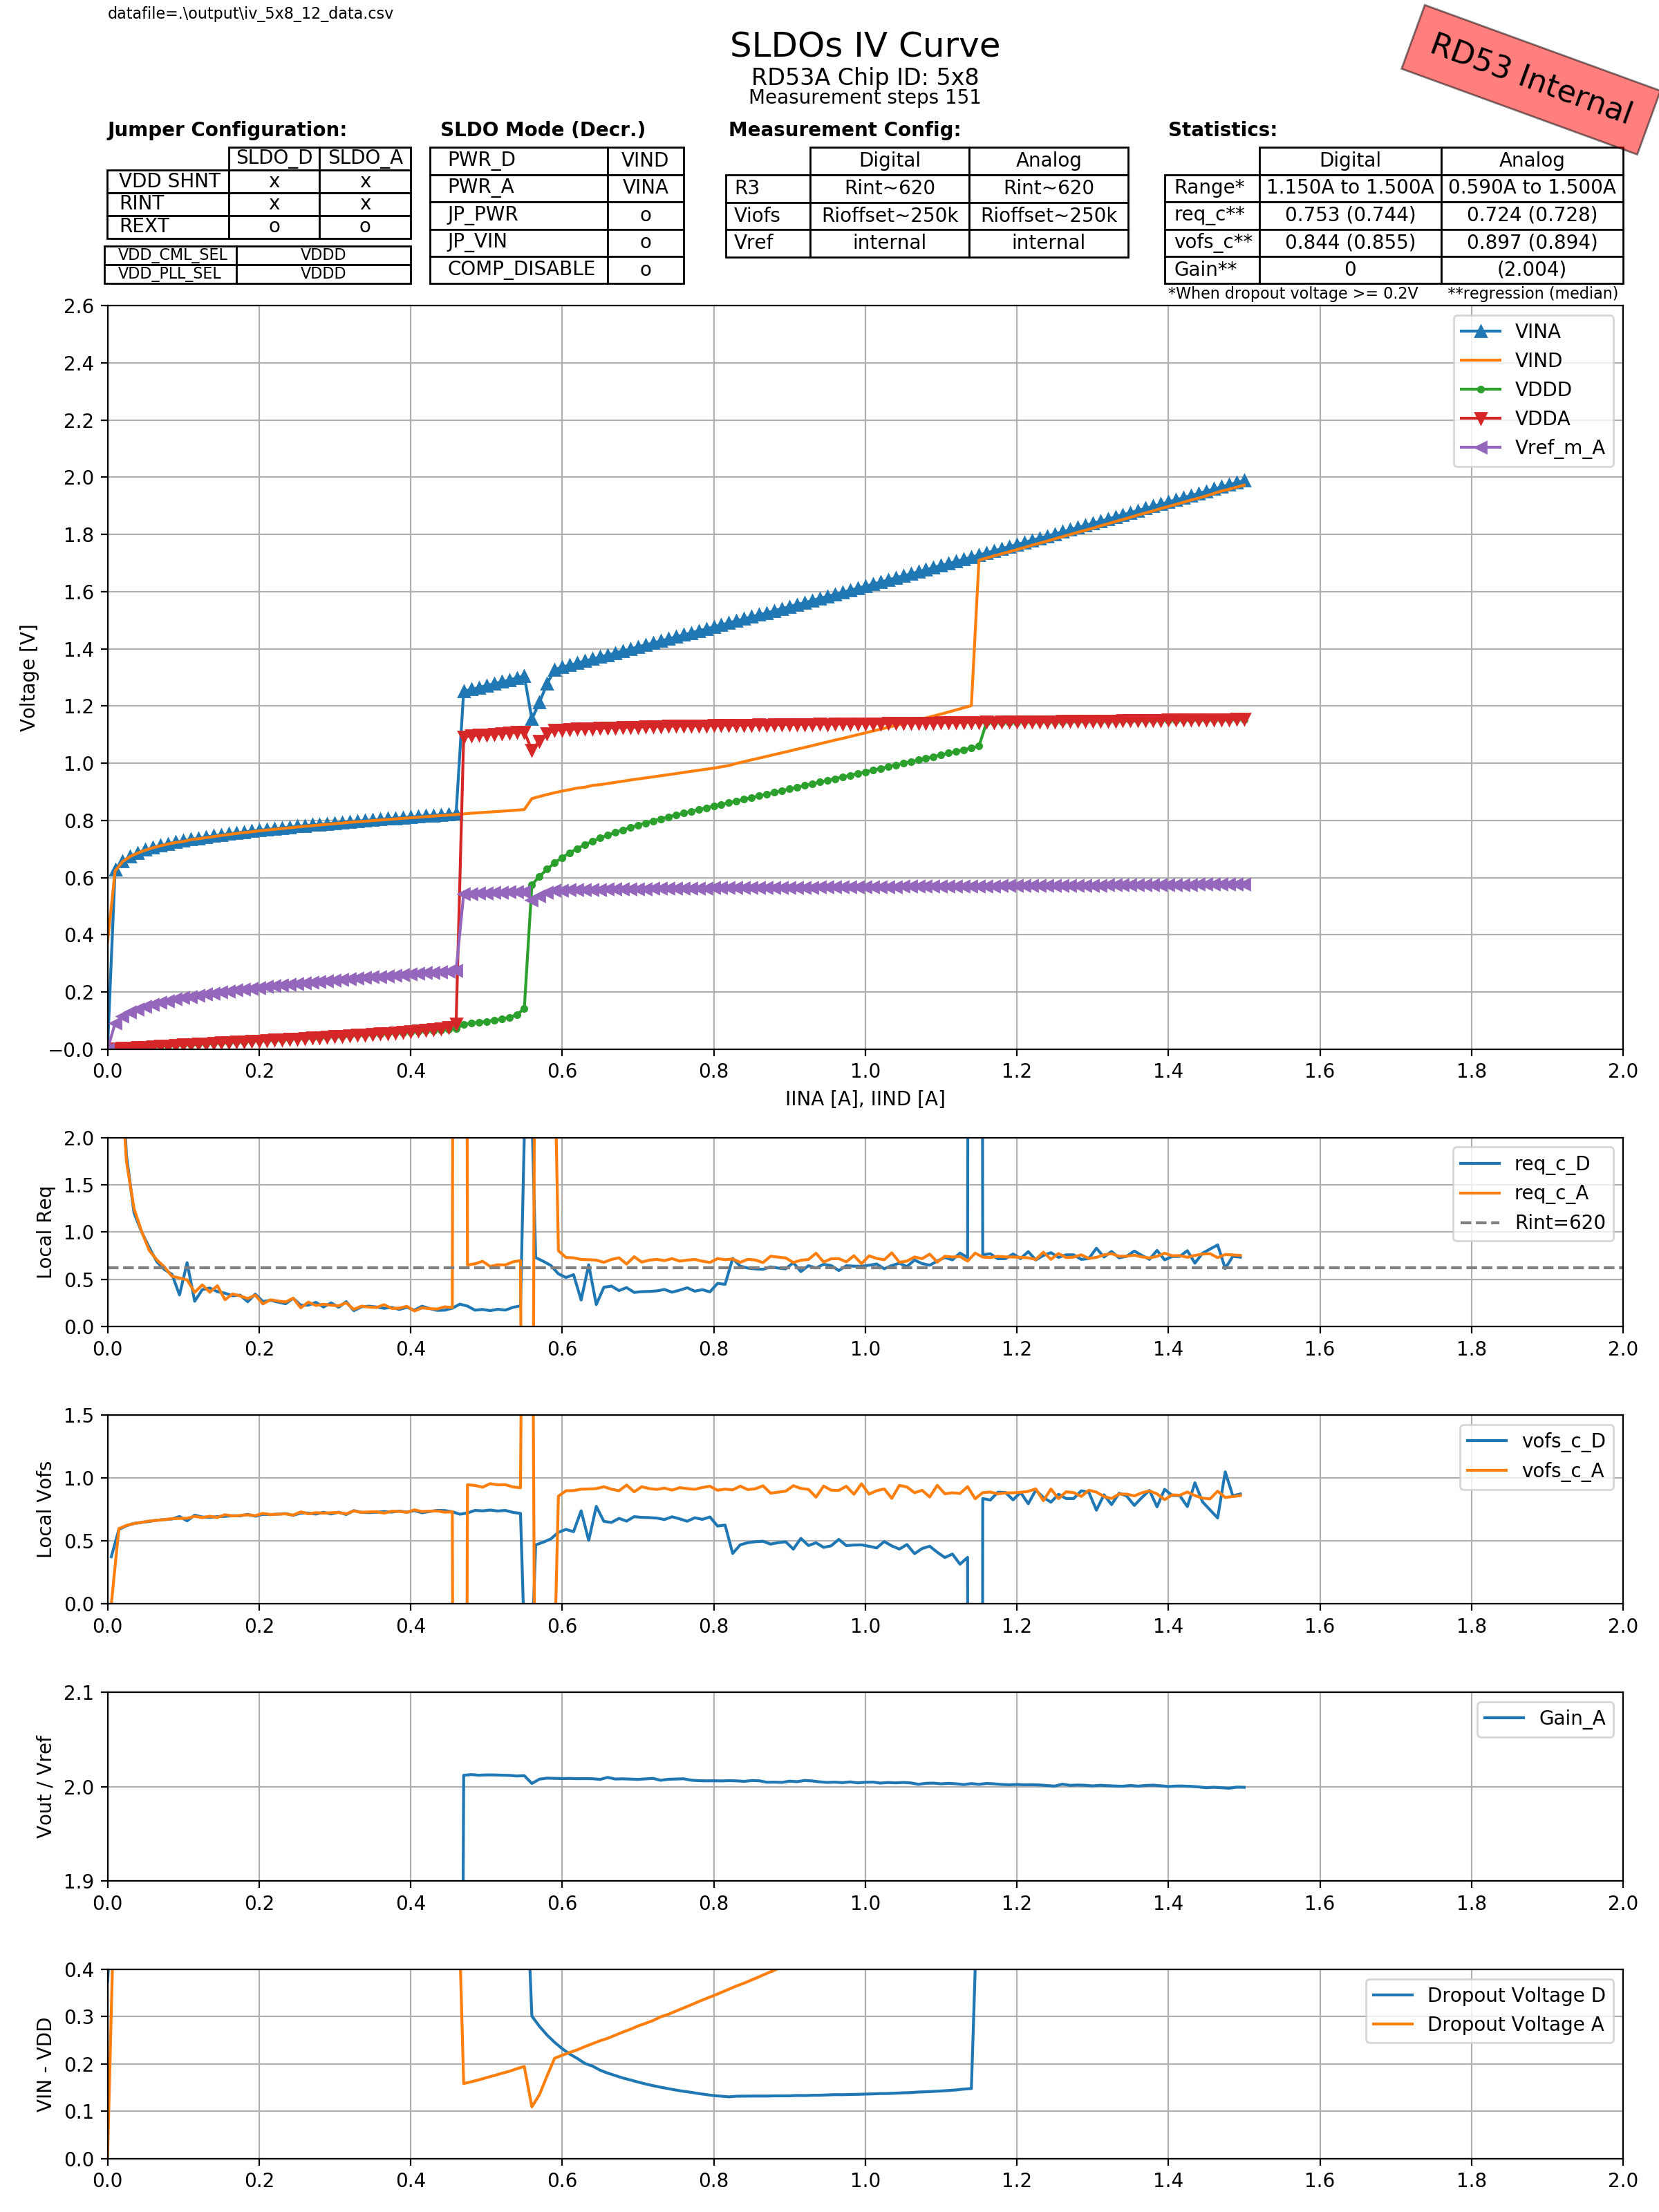
\includegraphics[scale=.3]{Immagini/iv_5x8_12_plt_01}
\caption{.}
\label{iv_5x8_12_plt_01}
\end{figure}



\subsection{LDOvsSLDO}

\begin{figure}
\centering
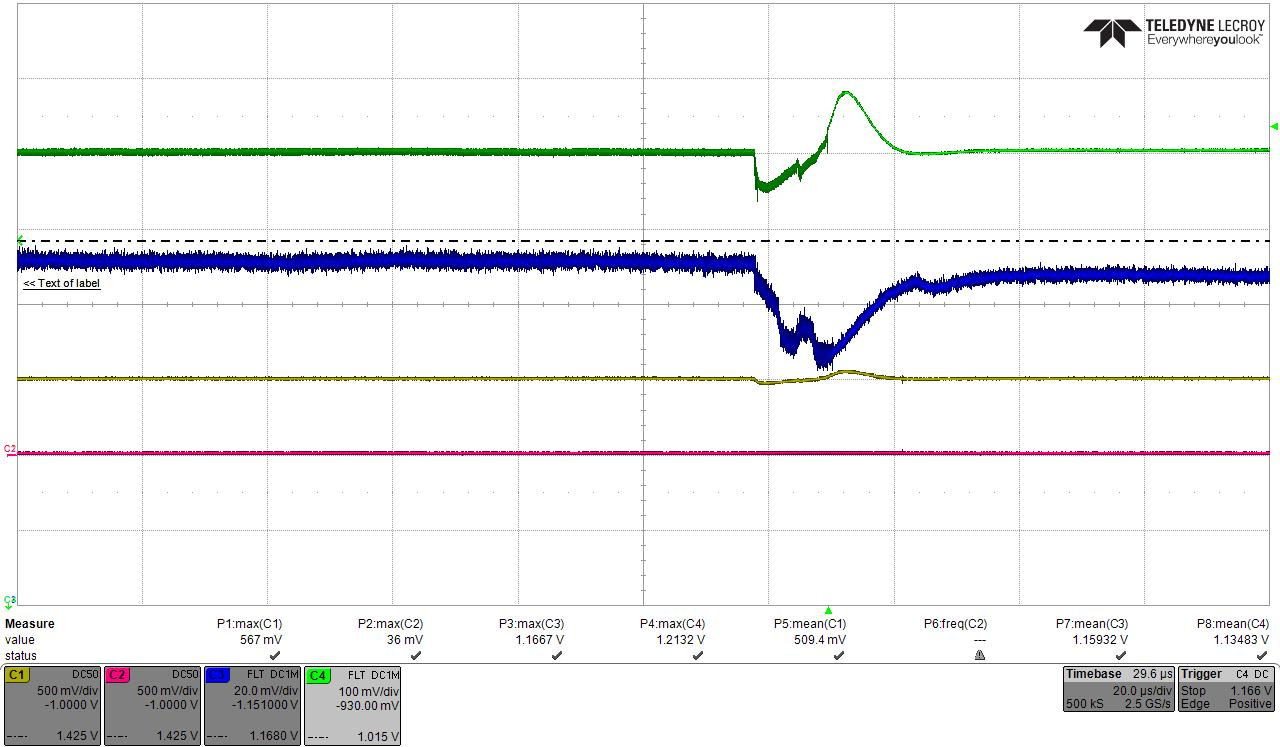
\includegraphics[scale=.3]{Immagini/alllin1}
\caption{.}
\label{alllin1}
\end{figure}


\section{Front End}
\subsubsection{Torino}
\subsubsection{LBNL}
\subsubsection{Bonn}
\section{Sistemi di acquisizione dati}
\section{Setup}

%3.3 ESD Protection and Safe Wire Bonding
%
%%In the bottom pad frame the four power domains (VDDA, VDDD, VDD_CML, and VDD_PLL) are
%isolated by power-cut cells. Within a power domain group, the IO pad ESD devices are connected
%to the respective power rails. To allow an ESD path between power domains a common ESD
%bus connects to every power domain’s ground rail via sets of anti-parallel diodes. This ESD bus
%is also used to connect the global substrate of the chip (VSUB). !!!!!!Because the IO pads use ESD
%devices connecting to the power rails, care must be taken to not drive signals to the chip while it
%is not powered, as this would supply parasitic power. There are a few pads which have an over-
%voltage tolerant ESD protection without a current path to the power rail. These pads are used where
%the input voltage can exceed the VDDA/VDDD rail potentials (input- and bias pads of the shunt
%regulator blocks, for example). Where low capacitance is mandatory (CML driver output pads) a
%path to the VDDA/VDDD rails was also omitted.
%%The top test pads have an independent power domain (VDD_TOP/GND_TOP) which is not
%connected to the global ESD bus at the chip bottom. Within the top row the IO pads are protected
%but since there is no connection to the global ESD bus, ESD events between top and bottom pads
%should be avoided. The IO pads in the top pad frame are all over-voltage tolerant and therefore
%output signals are not clamped if the top row is not powered.
%The wire bonding sequence to avoid ESD problems is as follows: Start with the VSUB pads
%(14, 88 and 184) followed by all GND pads in any order. Finally bond the remaining pads in any
%order. The top row pads can be left floating, but if wire bonded then start with the GND pads (T2,
%T51 and T97) followed by the VDD pads (T1, T50 and T96) and then all other pads.
\section{Scansioni}
